\chapter{Desarrollo del trabajo}  
%\addcontentsline{toc}{chapter}{\numberline{}Desarrollo del trabajo}

\section{Arquitectura y diseño de base de datos}

\subsection{Base de datos}

A continuación, se expone el diseño de la base de datos de cada perfil de usuario.

\begin{itemize}
	\item \texttt{configuration}: Es la única entidad sin relaciones con otras tablas. Tiene dos elementos, \texttt{key} y \texttt{value}. \todo
	\item \texttt{language}: Contiene información sobre los idiomas que el usuario está estudiando. Tiene los siguientes atributos:
		\begin{itemize}[label=$\star$]
			\item \texttt{id}: Identificador único del idioma.
			\item \texttt{name}: Nombre del idioma.
			\item \texttt{dictionary\_url}: URL al diccionario \textit{online} que se incrusta debajo del formulario de edición de los datos de palabras.
			\item \texttt{should\_show\_spaces}: Si tiene valor $1$, los espacios que contenga un texto se renderizarán con normalidad; en cambio, si tiene valor $0$, los espacios serán invisibles. Esto resulta útil en el caso de idiomas que no suelen separar las palabras mediante espacio, como el japonés o los idiomas chinos, para que, aunque la aplicación requiera algún carácter entre las distintas palabras para su correcto funcionamiento, esto no afecte negativamente a la experiencia del usuario.
			\item \texttt{alphabet}: Expresión regular que describe los caracteres que conforman las palabras del idioma.
			\item \texttt{sentence\_delimiters}: Expresión regular que describe los caracteres que denotan el final de un enunciado en el idioma.
			\item \texttt{whitespaces}: Expresión regular que describe los caracteres que denotan la separación entre palabras.
			\item \texttt{intraword\_punctuation}: Expresión regular que describe los caracteres que, aun no siendo parte del alfabeto, pueden aparecer en medio de una palabra.
			\item \texttt{template\_code}: Identificador de la plantilla utilizada como base para configurar el idioma.
			\item \texttt{script\_name}: \todo
			\item \texttt{text\_processors}: Lista de procesadores de texto que se ejecutan al importar textos en este idioma.
			\item \texttt{word\_data\_provider}: Proveedor de datos de palabras que se utilizará para autocompletar el formulario de modificación de palabra cuando se consulte una nueva palabra en este idioma.
		\end{itemize}
	\item \texttt{word}: Contiene información acerca de las palabras alguna vez vistas por el usuario. Contiene los siguientes atributos:
	\begin{itemize}[label=$\star$]
		\item \texttt{id}: Identificador único de la palabra.
		\item \texttt{language\_id}: Identificador del idioma al que pertenece la palabra.
		\item \texttt{content}: Secuencia de caracteres que conforman la palabra.
		\item \texttt{status}: Nivel de familiarización del usuario con la palabra. Vale $1$ para palabras que el usuario solo haya visto una vez, y aumenta gradualmente hasta $5$ para palabras que sean prácticamente del todo familiares para el usuario. Una vez el usuario marque la palabra como aprendida, el valor de \texttt{status} será $99$. Se reserva el valor $98$ para palabras que deben ser ignoradas: según la metodología del estudiante, puede usarse para nombres propios, para palabras inexistentes (que pueden emerger con motivo del funcionamiento imperfecto de los analizadores sintácticos) o para palabras que no pertenecen al idioma en cuestión.
		\item \texttt{notes}: Anotaciones sobre la palabra.
		\item \texttt{time\_added}: \textit{Timestamp} del momento de creación de la palabra.
		\item \texttt{time\_updated}: \textit{Timestamp} del momento de última actualización de la palabra.
		\item \texttt{token\_count}: Número de \textit{tokens} que conforman la palabra. Es útil para formas complejas como locuciones, que están formadas por varias palabras pero actúan para muchos efectos como una sola.
	\end{itemize}
	\item \texttt{entry}: Entrada de diccionario de una palabra.
	\begin{itemize}[label=$\star$]
		\item \texttt{id}: Identificador único de la entrada.
		\item \texttt{word\_id}: Identificador de la palabra a la que corresponde la entrada.
		\item \texttt{position}: Posición en la que se coloca la entrada.
		\item \texttt{meaning}: Acepciones de la palabra según esta entrada.
		\item \texttt{reading}: Lectura de la palabra según esta entrada.
	\end{itemize}
	\item \texttt{word\_status\_log}: Histórico de cambios realizados al estado de las palabra.
	\begin{itemize}[label=$\star$]
		\item \texttt{id}: Identificador único del cambio.
		\item \texttt{word\_id}: Identificador de la palabra a la que corresponde el cambio.
		\item \texttt{status}: Nuevo estado de la palabra.
		\item \texttt{time\_updated}: \textit{Timestamp} del momento en que se realizó el cambio.
	\end{itemize}
	\item \texttt{text}: Contiene información acerca de un texto.
	\begin{itemize}[label=$\star$]
		\item \texttt{id}: Identificador único del texto.
		\item \texttt{language\_id}: Identificador del idioma en que está escrito el texto.
		\item \texttt{title}: Título del texto.
		\item \texttt{source\_url}: URL de la página web de la que se importó el texto, en caso de que aplique.
		\item \texttt{time\_opened}: \textit{Timestamp} del momento en que se abrió el texto por última vez.
		\item \texttt{time\_finished}: \textit{Timestamp} del momento en que se terminó de leer el texto por completo.
		\item \texttt{progress}: Valor entre $0$ y $1$ que indica el porcentaje de páginas del texto que el usuario ha leído.
	\end{itemize}
	\item \texttt{page}: Página de un texto.
	\begin{itemize}[label=$\star$]
		\item \texttt{id}: Identificador único de la página.
		\item \texttt{text\_id}: Identificador del texto al que pertenece la página.
		\item \texttt{position}: Posición en la que se coloca la página.
		\item \texttt{content}: Contenido de la página.
	\end{itemize}
	\item \texttt{text\_progress\_log}: Histórico de cambios realizados al progreso de un texto.
	\begin{itemize}[label=$\star$]
		\item \texttt{id}: Identificador único del cambio.
		\item \texttt{text\_id}: Identificador del texto al que corresponde el cambio.
		\item \texttt{progress}: Nuevo progreso de la palabra.
		\item \texttt{time\_updated}: \textit{Timestamp} del momento en que se realizó el cambio.
	\end{itemize}
\end{itemize}

\begin{figure}
	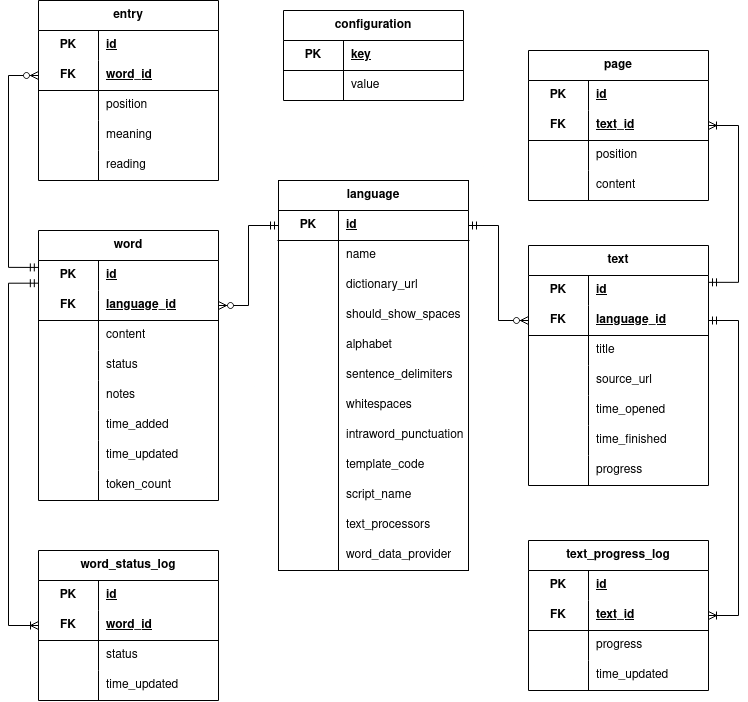
\includegraphics[width=1\textwidth]{er-diagram.drawio.png}
	\caption[Diagrama entidad-relación]{Diagrama entidad-relación con notación \textit{Crow's foot}.}
\end{figure}

\subsection{Sistema de \textit{plugins}}

Para hacer posible el estudio de cualquier idioma, y como solicita la historia de usuario 2.1, se implementó un sistema de \textit{plugins} para modificar el funcionamiento de la aplicación según necesidades particulares de los usuarios.

Existen dos tipos de funcionalidades que pueden implementar los \textit{plugins}:
\begin{itemize}
	\item \textbf{Procesadores de texto}: Se pueden llamar en el momento de importar un nuevo texto en la base de datos. Su objetivo es \textit{interceptar} el texto a importar y manipularlo según esté programado en el código del \textit{plugin}. Se proponen algunos casos de uso para este tipo de funcionalidad, y en el anexo se incluye el código correspondiente.
	\begin{itemize}[label=$\star$]
		\item Insertar caracteres de separación de palabras para idiomas que no utilicen espacios, como el japonés o los idiomas chinos.
		\item Eliminar anotaciones irrelevantes para el usuario al importar texto de un formato distinto al texto plano, como el formato SRT para subtítulos.
		\item Transformar el texto a otro sistema de escritura en el caso de idiomas que utilicen varios, como el serbio, que puede ser escrito tanto con el alfabeto cirílico como con el latino.
	\end{itemize}
	\item \textbf{Proveedores de datos de palabras}: Se pueden llamar al clicar sobre una palabra nueva para autocompletar el formulario de los datos sobre la palabra, de forma que el usuario no tenga que copiar manualmente las definiciones desde un diccionario.
\end{itemize}

Para ello, se creó una clase \texttt{PluginManager} que, como su nombre indica, gestiona la ejecución de los \textit{plugins} que cargue el usuario. Esta clase contiene un objeto \texttt{PluginManager.api}, que de manera simplificada tiene tres métodos:

\begin{itemize}
	\item \texttt{register}, para registrar un \textit{plugin}.
	\item \texttt{registerTextProcessor}, para registrar un procesador de texto.
	\item \texttt{registerWordDataProvider}, para registrar un proveedor de datos de palabras. \todo (Pensar un mejor nombre).	
\end{itemize}

El \texttt{PluginManager} almacena un \textit{array} de todos los plugins registrados.

Los \textit{plugins} se ejecutan mediante el método \texttt{AsyncLocalStorage.run} de Node, que se encarga de separar el contexto del \textit{plugin} del del resto de la aplicación. Aunque estén en contextos distintos, el \textit{plugin} debe tener alguna forma de registrarse en el contexto principal. Para ello, antes de cargar los \textit{plugins}, se almacena una copia del objeto \texttt{PluginManager.api} en una variable global que después leerán los \textit{plugins}. Esta variable global se inicializa como un objeto \textit{proxy} que previene realizar modificaciones en la API.

\begin{center}
\begin{typescript}
const sandboxProxy = (target: any) => {
	const proxy = new Proxy(
		target,
		{
			get(target: any, property: string, receiver: any): any
			{
				if (property in target)
				{
					return Reflect.get(target, property, receiver);
				}
				else
				{
					throw new Error('Property ' + property + ' not found');
				}
			},
			set(target: any, property: string, value: any, receiver: any): any
			{
				throw new Error('Setting properties is not allowed');
			},
		}
	);
	
	return proxy;
};
\end{typescript}
\end{center}

Diagrama frontend vs backend, incluir sistema de archivos.

Todo con explicación, evidentemente.

\section{Diseño UI/UX}

Explicar diseño. Leyes Gestalt, teoría de colores y esas cosas. Diseño responsive también. Accesibilidad.

\section{Proceso de desarrollo}

Agile llevado a la práctica.

Decir algo sobre \textit{feedback}.
